\documentclass{article}
\usepackage{graphicx}
\usepackage{amsmath}
\usepackage{enumitem}
\usepackage{float}
\usepackage{listings}
\usepackage{xcolor}
\usepackage[a4paper, margin=1in]{geometry}

% Custom information
\newcommand{\className}{Course: Automatic Control Systems – ASEN 5114-001 – Spring 2025}
\newcommand{\professorName}{Professor: Dale Lawrence}
\newcommand{\taName}{Teaching Assistant: Anantha Dhruva}
\title{Homework 2 \\ \className \\ \professorName \\ \taName}
\author{Steve Gillet}
\date{\today}

\lstdefinestyle{matlabstyle}{
    language=Matlab,              % Specify the language
    basicstyle=\ttfamily\footnotesize\color{black}, % Code font
    keywordstyle=\color{blue}\bfseries, % Keywords in blue
    stringstyle=\color{orange},    % Strings in green
    commentstyle=\color{magenta}, % Comments in magenta
    numbers=left,                 % Line numbers on the left
    numberstyle=\tiny\color{black},% Line number style
    stepnumber=1,                 % Line number increment
    breaklines=true,              % Line breaking
    frame=single,                 % Border around code
    backgroundcolor=\color{white},
    tabsize=4,                    % Tab size
    showstringspaces=false,       % Don't show spaces in strings
}

\begin{document}

\maketitle
\textit{
    "Use the plant and controller models from Homework 1 to explore the effect of control gains on
    closed loop system poles, and hence the effect on the closed loop natural response of the load
    shaft angle."
}

\section*{1.}

\textit{
    "Find the poles of the plant from your transfer function model from Experiment 1. Plot these
    in the complex plane."
}

This is the Matlab code I used to get the roots of my Open Loop Transfer Function using 'roots' Matlab function.

\begin{lstlisting}[style=matlabstyle]
coeff3=0.000028291; % [Vs^3]
coeff2=0.285890679; % [Vs^2]
coeff1=1.332; % [Vs/rad]
num = [-1];
den = [coeff3, coeff2, coeff1, 0];
format longG;
poles = roots(den);
disp(poles);

figure;
plot(real(poles), imag(poles), 'x', 'MarkerSize', 10, 'LineWidth', 2);
title('Open Loop Poles');
xlabel('Re');
ylabel('Im');
grid on;
\end{lstlisting}

You can just feed the coefficients into that function and it will get the roots of that polynomial for you and then I graphed the real and imaginary components using 'real' and 'imag' functions and the results are below.

\begin{figure}[H]
    \centering
    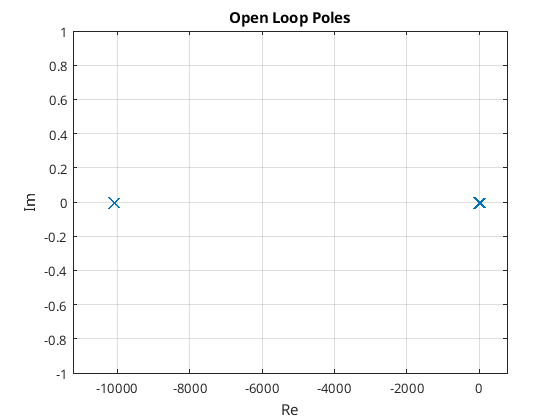
\includegraphics[width=\textwidth]{openPolesZoomedOut.png}
\end{figure}
\begin{figure}[H]
    \centering
    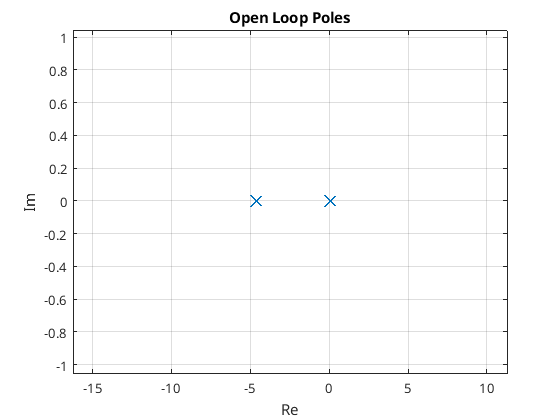
\includegraphics[width=\textwidth]{openPolesZoomedIn.png}
\end{figure}

I had to take one picture zoomed out and then one zoomed in because the roots were 0, -4.66127366088196, and -10100.6965786596 and when the graph is zoomed out enough to see -10,100 you can't distinguish 0 and -4.66.

\section*{2.}

\textit{
    "Find the poles of the closed loop system from part 5 of Homework 1. Plot these on the same
    plot as in part 1. above."
}

I used the same technique as for the open loop except the gains were added in of course.

\begin{lstlisting}[style=matlabstyle]    
Gp = -10;
Gd = -0.1;
numCL = [-Gd -Gp];
denCL = [coeff3, coeff2, coeff1 - Gd, -Gp];
polesCL = roots(denCL);
disp(polesCL);

plot(real(polesCL), imag(polesCL), 'rx', 'MarkerSize', 10, 'LineWidth', 2);
legend('Open Loop Poles', 'Closed Loop Poles');
\end{lstlisting}

I plotted the closed loop poles (red) on top of the open loop poles (blue) and the results are below.

\begin{figure}[H]
    \centering
    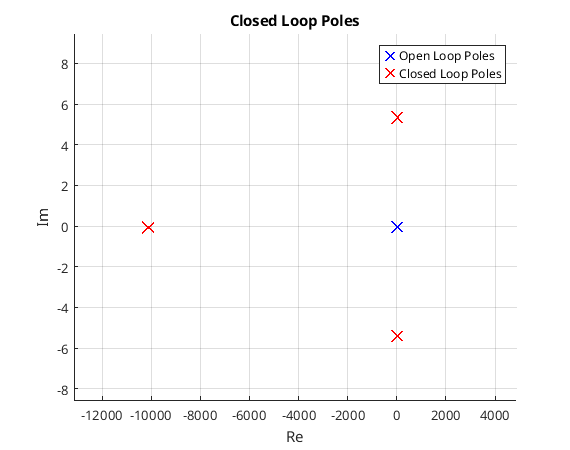
\includegraphics[width=\textwidth]{closedPoles.png}
\end{figure}

The -10100 open loop pole is still there but you have to zoom in to see it since the closed loop is basically right on top of it.
    
\section*{3.}

\textit{
    "Repeat part 2. above, using a gain factor g in the control law that varies between 0 and 1, in
    100 steps. Plot this 'root locus with respect to g' on the same plot as above. Describe the
    effect of this control system gain on the closed loop poles."
}

I accomplished this with a scaling variable and a for loop.

\begin{lstlisting}[style=matlabstyle]    
gScalar = linspace(0, 1, 100);
for i = 1:length(gScalar)
    g = gScalar(i);
    denCL = [coeff3, coeff2, coeff1 - Gd*g, -Gp*g];
    polesCL = roots(denCL);
    plot(real(polesCL), imag(polesCL), 'k.', 'MarkerSize', 1);
    disp(polesCL);
end

legend('Open Loop Poles', 'Closed Loop Poles', 'Root Locus');
\end{lstlisting}

What you see on the plot and in the values of the poles is that when the gains are scaled to 0 the closed loop poles become the open loop poles and then as you scale them up to their full value they move out towards their closed loop values.

\begin{figure}[H]
    \centering
    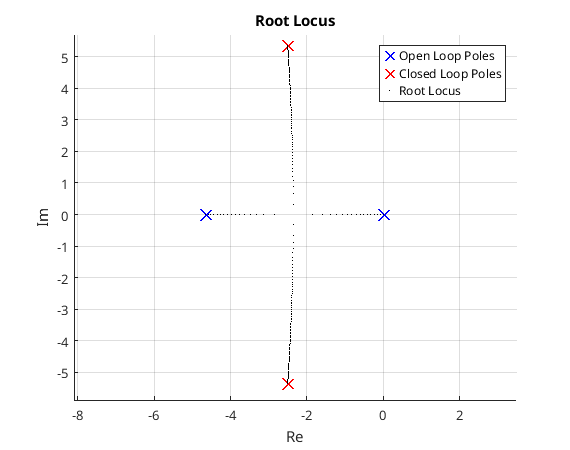
\includegraphics[width=\textwidth]{rootLocus.png}
\end{figure}
\begin{figure}[H]
    \centering
    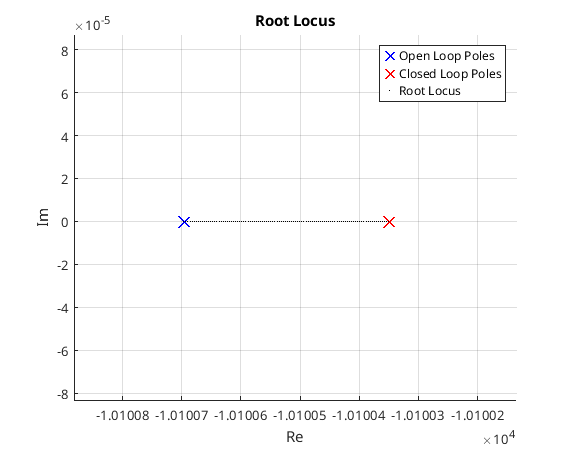
\includegraphics[width=\textwidth]{rootLocusBigNeg.png}
\end{figure}

\section*{4.}

\textit{
    "Repeat part 3. above but use gain values g between 1 and 100. Describe the effect on the
    closed loop poles."
}

\begin{figure}[H]
    \centering
    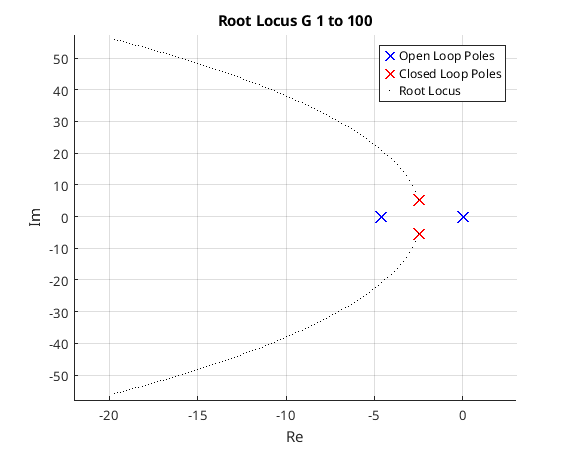
\includegraphics[width=\textwidth]{rootLocus100.png}
\end{figure}
\begin{figure}[H]
    \centering
    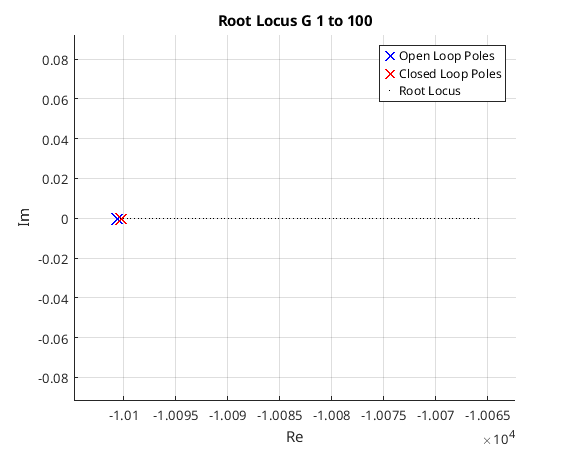
\includegraphics[width=\textwidth]{rootLocus100bigNeg.png}
\end{figure}

The imaginary poles grew larger in the imaginary axis and more negative in the real axis.
This is going to have the effect of increasing the frequency of the response and decreasing the settling time.
The real pole also shifted slightly towards the origin as the gains increased, although it was very small I don't think this means that it would ever actually go towards the origin or converge to the other poles.

\section*{5.}

\textit{
    "Repeat part 4. but use negative g values between 0 and -1."
}

\begin{figure}[H]
    \centering
    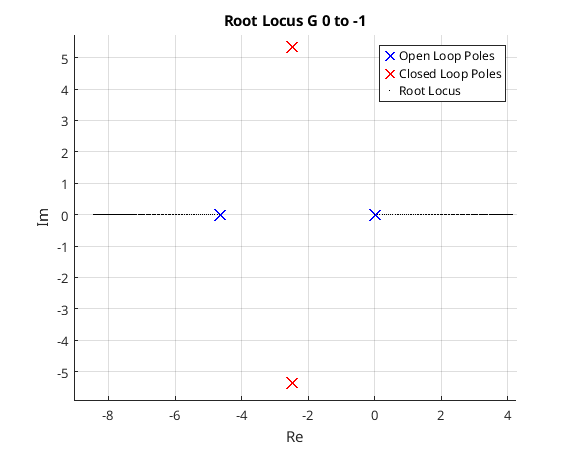
\includegraphics[width=\textwidth]{rootLocusNegativeG.png}
\end{figure}

Making those gains negative pushed all of the open loop poles away from the origin, which had the unfortunate effect of creating a positive pole which will create an explosive, unstable behavior.
There's this interesting overall trend where the negative gain (overall positive) closed loop poles have large real values and then as the gains go positive (negative overall) the poles converge towards -2.2 real value and then become imaginary and move back out away from the origin again increasing in real and imaginary axes.

\section*{6.}

\textit{
    "What does the above root locus analysis tell you about the effect of the gain g on the closed
    loop system’s natural response? Verify your conclusions by simulating the closed loop step
    response for several values for g."
}

I basically said it above already but I think the larger positive gain scaler is going to make the natural response have a higher frequency and converge faster and the negative g is going to make the natural response explode.
I used simulink to simulate a step response with 100, 10, 1, and -1 g gain scaler, the results are below.

\begin{figure}[H]
    \centering
    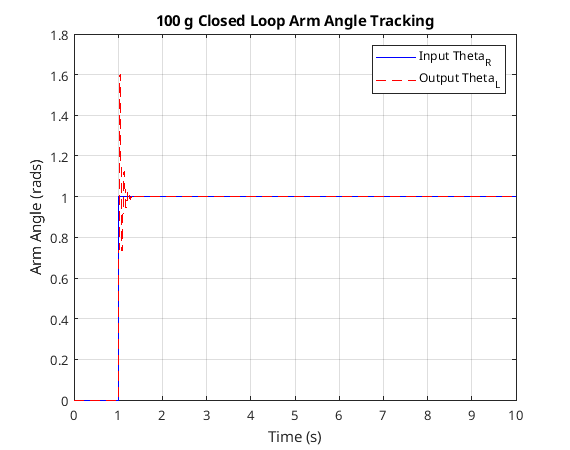
\includegraphics[width=\textwidth]{100gStep.png}
\end{figure}
\begin{figure}[H]
    \centering
    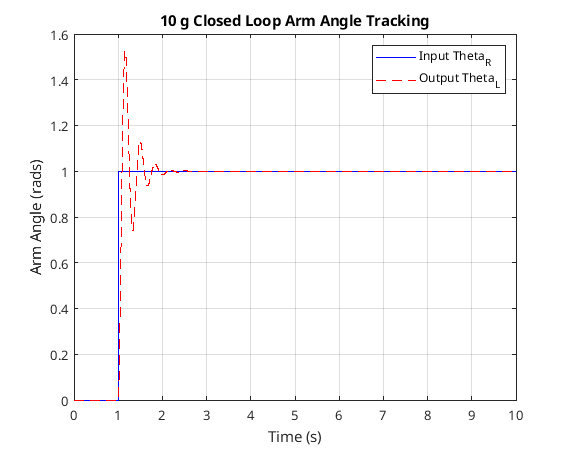
\includegraphics[width=\textwidth]{10gStep.png}
\end{figure}
\begin{figure}[H]
    \centering
    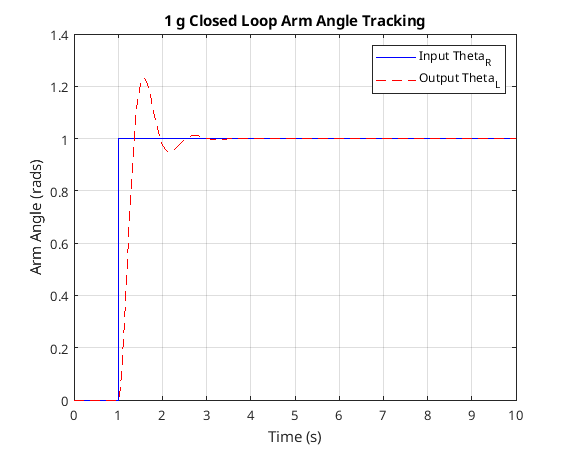
\includegraphics[width=\textwidth]{1gStep.png}
\end{figure}
\begin{figure}[H]
    \centering
    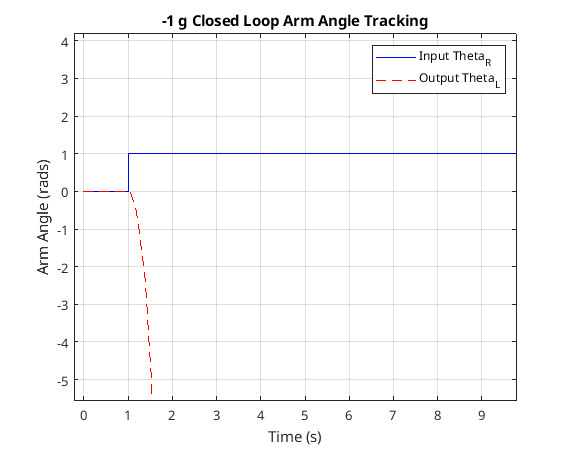
\includegraphics[width=\textwidth]{-1gStep.png}
\end{figure}

I believe this shows my predictions to be correct.
You can see the faster oscillations and quicker settling time as g is higher, when g is 100 the response settles in a third of a second and when g is 1 it takes about 3 seconds.
I do think it is worth pointing out that the amplitude is also a bit higher when g is higher which I did not mention or predict before.

\end{document}